% Membuat gambar contoh (data fiktif untuk ilustrasi format): alur-penelitian, topologi, grafik-throughput, grafik-fairness
\documentclass[multi=tikzpicture,border=4pt]{standalone}
\usepackage{fontspec}
\IfFontExistsTF{Times New Roman}{\setmainfont{Times New Roman}}{\setmainfont{TeX Gyre Termes}}
\usepackage{tikz,pgfplots}
\pgfplotsset{compat=1.17}
\usetikzlibrary{shapes.geometric,arrows.meta,positioning,calc}
\begin{document}
% ---------- 1. Alur penelitian ----------
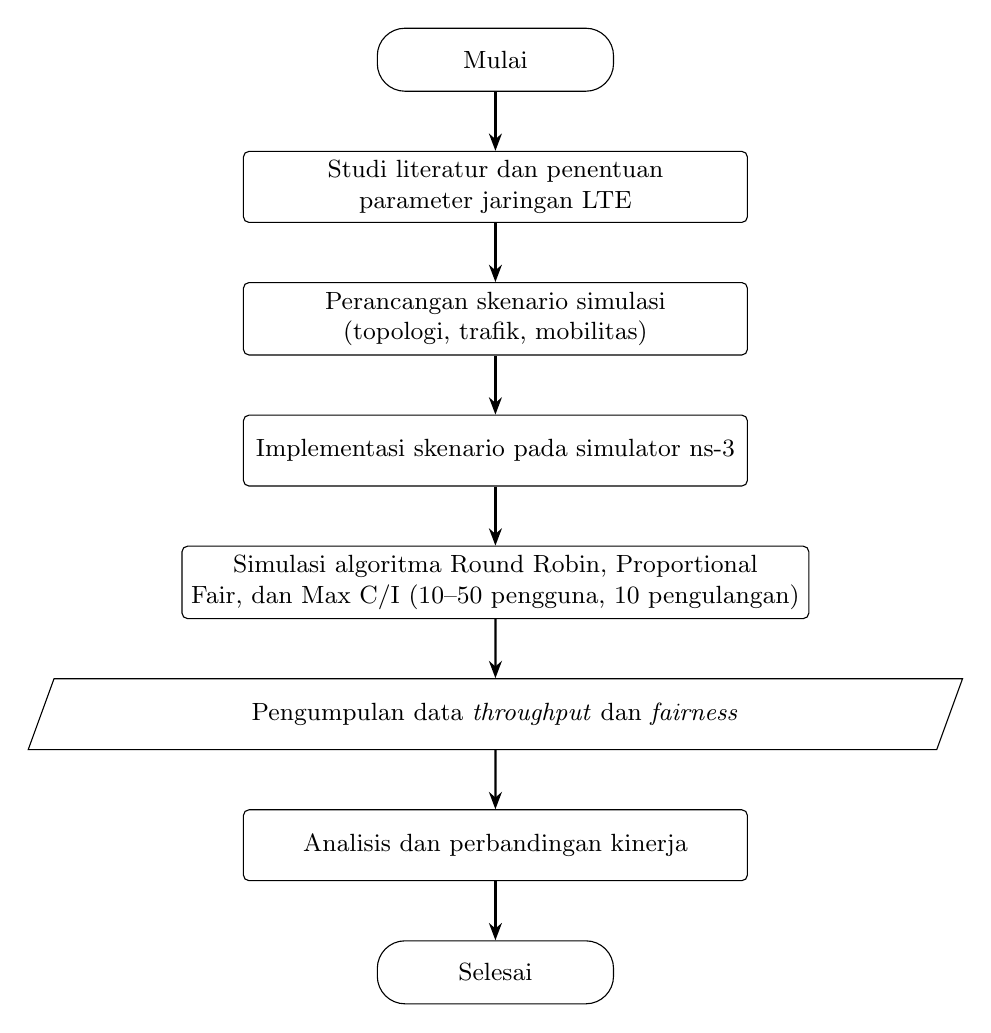
\begin{tikzpicture}[node distance=0.75cm,
  proses/.style={draw,rectangle,rounded corners=2pt,minimum width=6.4cm,minimum height=0.9cm,align=center,font=\small},
  term/.style={draw,rectangle,rounded corners=10pt,minimum width=3cm,minimum height=0.8cm,font=\small},
  io/.style={draw,trapezium,trapezium left angle=70,trapezium right angle=110,minimum width=6.4cm,minimum height=0.9cm,align=center,font=\small},
  panah/.style={-{Stealth[length=2.2mm]},thick}]
\node[term] (a) {Mulai};
\node[proses,below=of a] (b) {Studi literatur dan penentuan\\ parameter jaringan LTE};
\node[proses,below=of b] (c) {Perancangan skenario simulasi\\ (topologi, trafik, mobilitas)};
\node[proses,below=of c] (d) {Implementasi skenario pada simulator ns-3};
\node[proses,below=of d] (e) {Simulasi algoritma Round Robin, Proportional\\ Fair, dan Max C/I (10--50 pengguna, 10 pengulangan)};
\node[io,below=of e] (f) {Pengumpulan data \textit{throughput} dan \textit{fairness}};
\node[proses,below=of f] (g) {Analisis dan perbandingan kinerja};
\node[term,below=of g] (h) {Selesai};
\foreach \i/\j in {a/b,b/c,c/d,d/e,e/f,f/g,g/h} \draw[panah] (\i) -- (\j);
\end{tikzpicture}
% ---------- 2. Topologi ----------
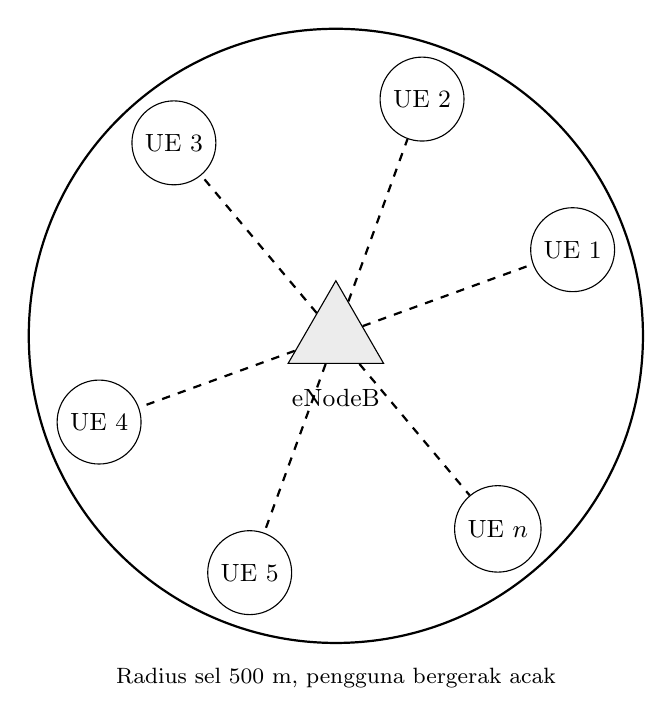
\begin{tikzpicture}[ue/.style={circle,draw,minimum size=0.8cm,font=\small},enb/.style={draw,regular polygon,regular polygon sides=3,minimum size=1.4cm,font=\small,fill=gray!15}]
\node[enb] (e) at (0,0) {};
\node[font=\small,below=0.2cm of e] {eNodeB};
\foreach \a/\n in {20/UE 1,70/UE 2,130/UE 3,200/UE 4,250/UE 5,310/UE $n$}{
  \node[ue] (u\a) at (\a:3.2cm) {\n};
  \draw[thick,dashed] (e) -- (u\a);
}
\draw[thick] (0,0) circle (3.9cm);
\node[font=\footnotesize] at (0,-4.35) {Radius sel 500 m, pengguna bergerak acak};
\end{tikzpicture}
% ---------- 3. Grafik throughput ----------
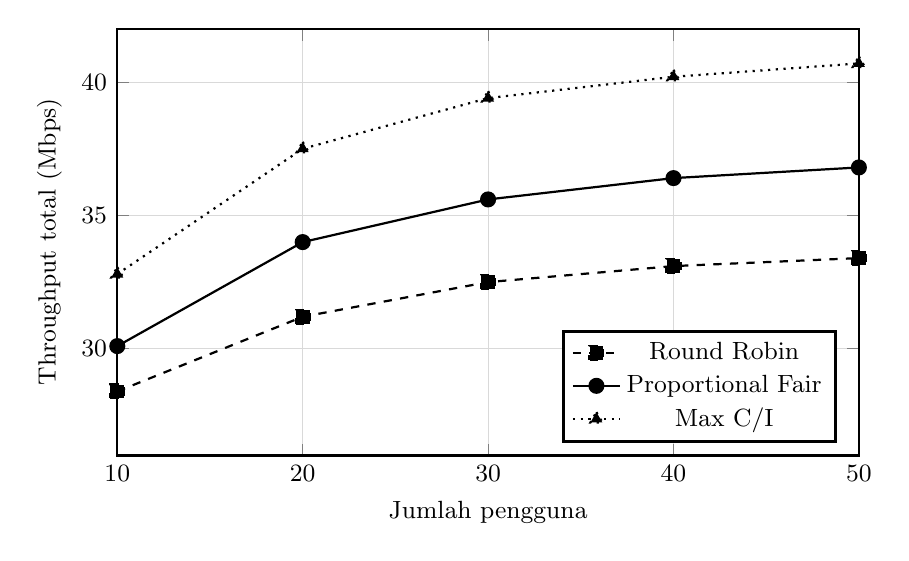
\begin{tikzpicture}
\begin{axis}[width=11cm,height=7cm,xlabel={Jumlah pengguna},ylabel={Throughput total (Mbps)},xmin=10,xmax=50,ymin=26,ymax=42,xtick={10,20,30,40,50},grid=major,grid style={gray!30},legend pos=south east,legend style={font=\small},tick label style={font=\small},label style={font=\small},mark size=2.5pt,thick]
\addplot[black,mark=square*,dashed] coordinates {(10,28.4)(20,31.2)(30,32.5)(40,33.1)(50,33.4)};
\addplot[black,mark=*] coordinates {(10,30.1)(20,34.0)(30,35.6)(40,36.4)(50,36.8)};
\addplot[black,mark=triangle*,dotted] coordinates {(10,32.8)(20,37.5)(30,39.4)(40,40.2)(50,40.7)};
\legend{Round Robin,Proportional Fair,Max C/I}
\end{axis}
\end{tikzpicture}
% ---------- 4. Grafik fairness ----------
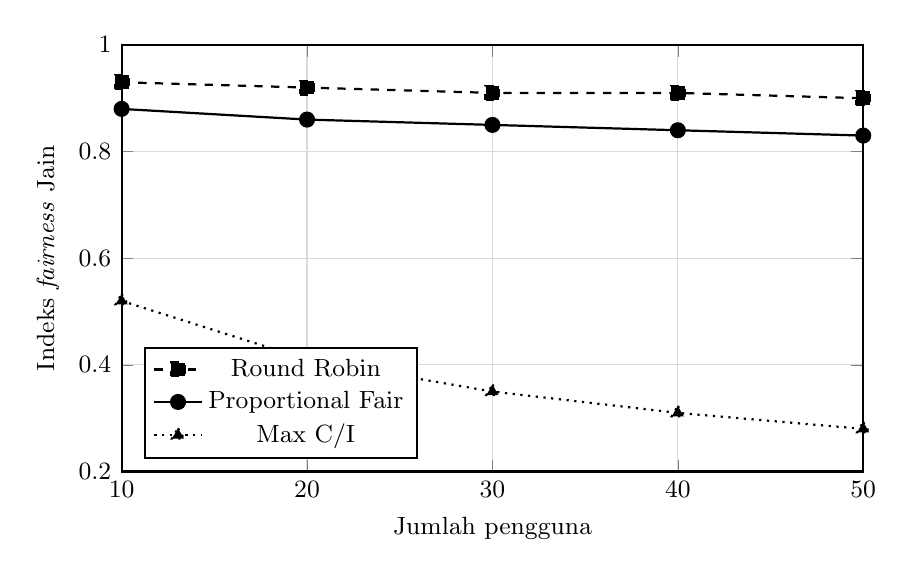
\begin{tikzpicture}
\begin{axis}[width=11cm,height=7cm,xlabel={Jumlah pengguna},ylabel={Indeks \textit{fairness} Jain},xmin=10,xmax=50,ymin=0.2,ymax=1.0,xtick={10,20,30,40,50},grid=major,grid style={gray!30},legend pos=south west,legend style={font=\small},tick label style={font=\small},label style={font=\small},mark size=2.5pt,thick]
\addplot[black,mark=square*,dashed] coordinates {(10,0.93)(20,0.92)(30,0.91)(40,0.91)(50,0.90)};
\addplot[black,mark=*] coordinates {(10,0.88)(20,0.86)(30,0.85)(40,0.84)(50,0.83)};
\addplot[black,mark=triangle*,dotted] coordinates {(10,0.52)(20,0.41)(30,0.35)(40,0.31)(50,0.28)};
\legend{Round Robin,Proportional Fair,Max C/I}
\end{axis}
\end{tikzpicture}
\end{document}
